\section{\ragname Framework}
\label{sec:framework}

\ragname is a claim-oriented verification-control framework for retrieval-augmented generation. 
% Given a query, the framework first obtains a draft answer from a plug-in RAG generator, converts the draft into atomic claims, constructs a claim-evidence coverage map, and iteratively uses verification signals to decide whether each claim should be kept, repaired, supported by additional retrieval, removed, or expressed as abstention. 
Section~\ref{subsec:framework_overview} gives the end-to-end overview. 
% Section~\ref{subsec:framework_overview} gives the end-to-end overview and formal controller. 
Section~\ref{subsec:framework_draft_decomp} describes how a plug-in draft generator is converted into claim-level units.
Section~\ref{subsec:framework_map} defines the claim-evidence coverage map. 
Section~\ref{subsec:framework_verification} specifies verification and label aggregation. 
Section~\ref{subsec:framework_control_repair} presents the control policy and targeted repair mechanism. 
Section~\ref{subsec:framework_final_audit} describes citation-constrained final generation and post-hoc audit.
% 中文：\ragname 是一个面向 retrieval-augmented generation 的 claim-oriented verification-control 框架。给定一个 query，框架首先从可插拔 RAG 生成器获得草稿答案，将草稿转换为原子 claims，构建 claim-evidence coverage map，并迭代地利用验证信号决定每个 claim 应该被保留、修复、通过额外检索补充证据、删除，还是表达为拒答。第~\ref{subsec:framework_overview} 节给出整体概览和形式化控制器；第~\ref{subsec:framework_draft_decomp} 节描述可插拔草稿生成器如何被转换为 claim-level units；第~\ref{subsec:framework_map} 节定义 claim-evidence coverage map；第~\ref{subsec:framework_verification} 节说明验证和标签聚合；第~\ref{subsec:framework_control_repair} 节给出控制策略和定向修复机制；第~\ref{subsec:framework_final_audit} 节描述带引用约束的最终生成和 post-hoc audit。

\begin{figure*}[t]
    \centering
    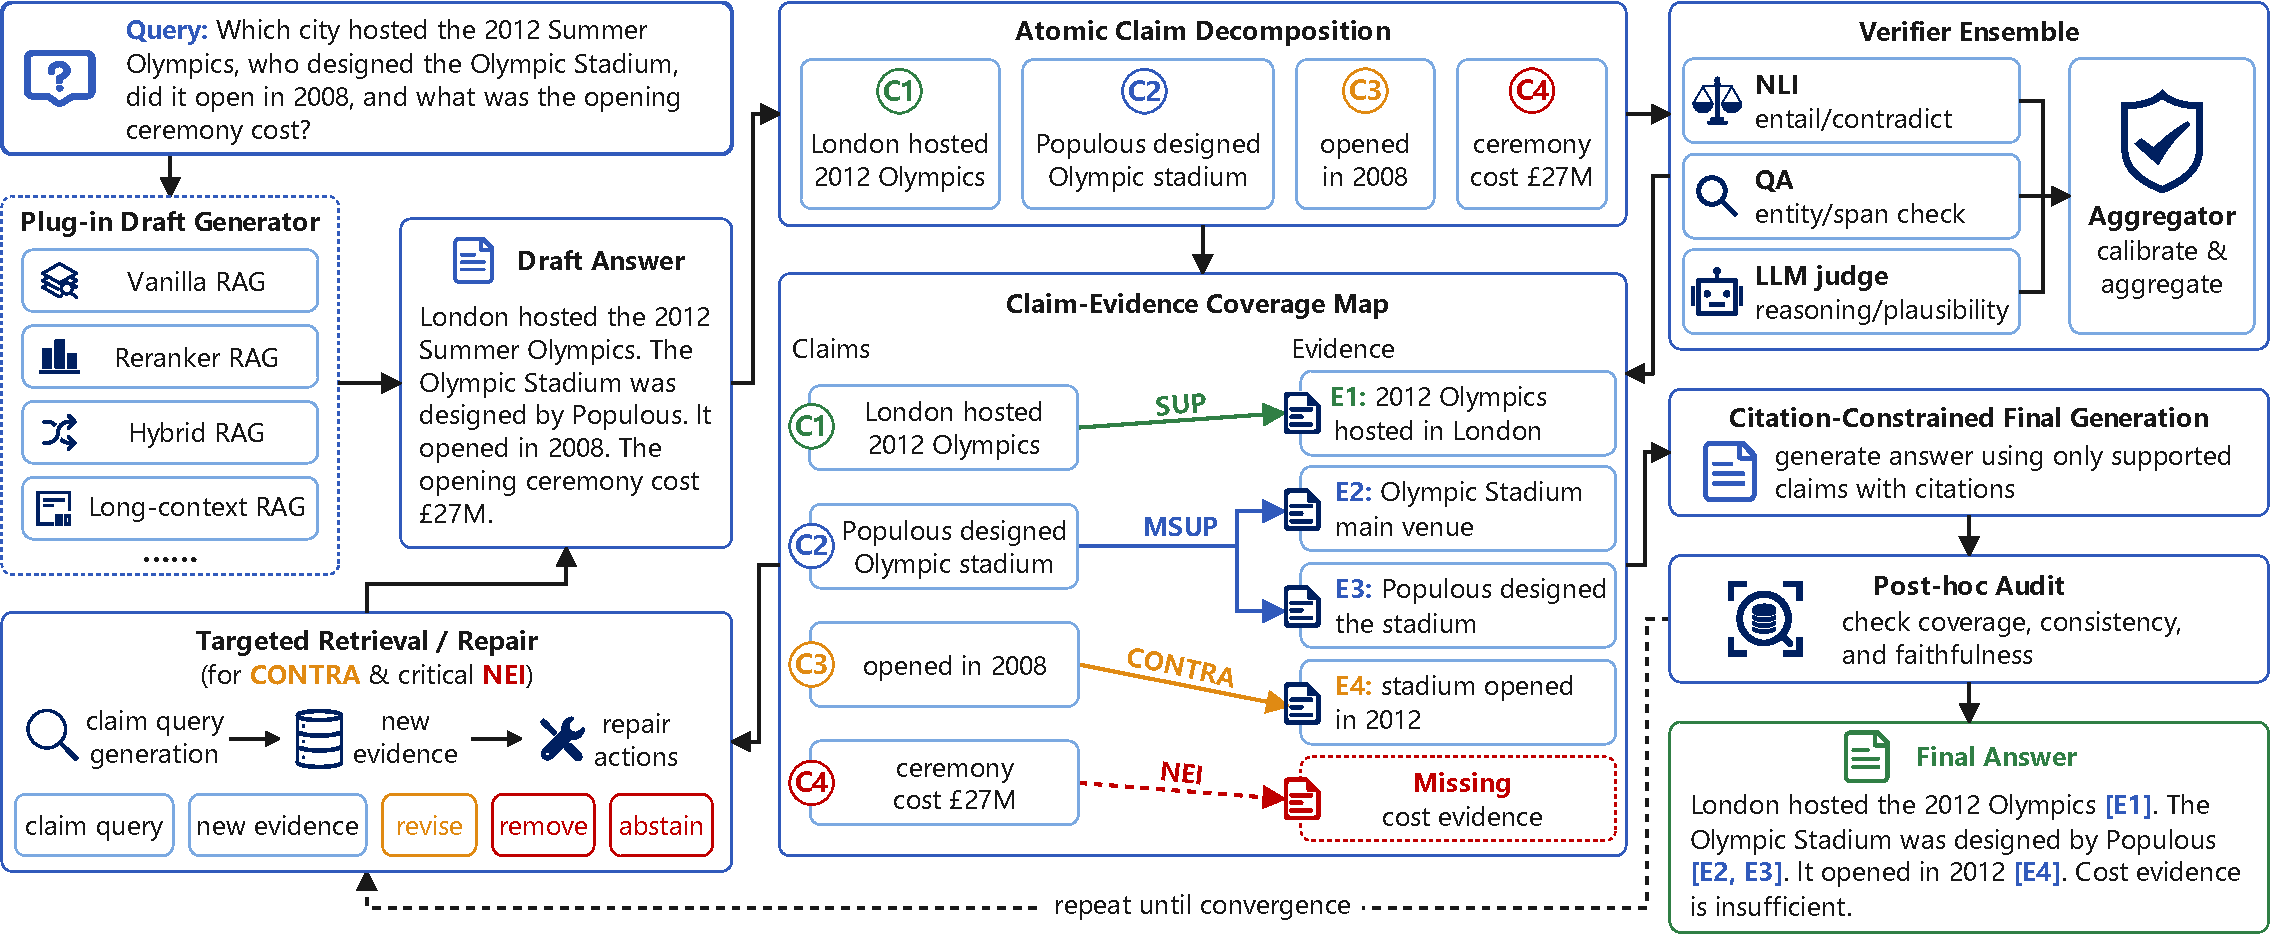
\includegraphics[width=\linewidth]{figs_wh/framework.pdf}
    \caption{Overview of the proposed \ragname framework. 
    % A plug-in RAG generator produces a draft answer, which is decomposed into atomic claims and organized into a claim-evidence coverage map. Verification labels drive targeted retrieval and repair until the map converges; the final answer is then generated under citation constraints and audited for residual unsupported claims.
    }
    % 中文图注：\ragname 总体框架。可插拔 RAG 生成器首先产生草稿答案，草稿被拆解为原子 claims，并组织为 claim-evidence coverage map。验证标签驱动定向检索和修复，直到 map 收敛；随后系统在引用约束下生成最终答案，并审计是否仍存在 unsupported claims。
    \label{fig:coverrag_framework}
\end{figure*}

\subsection{Overview}
\label{subsec:framework_overview}

\autoref{fig:coverrag_framework} gives the overall workflow of \ragname. 
% The framework starts from a user query and invokes a plug-in RAG generator to produce an initial draft answer. This draft is not treated as a final response, but as a structured hypothesis to be checked.
The framework first elicits an initial answer hypothesis from a plug-in proposal generator, which can be instantiated with any RAG backbone. This hypothesis is not used as the final response; instead, it is decomposed into atomic claims, organized into a claim-evidence coverage map, and used to control subsequent retrieval, verification, repair, and final generation.
% \ragname then decomposes the draft into atomic factual claims and associates each claim with candidate evidence. These claim-evidence associations form the coverage map, which becomes the working state of the framework.
% % 中文：图~\ref{fig:coverrag_framework} 给出了 \ragname 的整体工作流。框架从用户 query 开始，调用一个可插拔 RAG 生成器产生初始草稿答案。该草稿不是最终回答，而是一个需要被检查的结构化假设。随后，\ragname 将草稿拆解为原子事实 claims，并为每个 claim 关联候选证据。这些 claim-evidence associations 构成 coverage map，而该 map 成为整个框架的工作状态。

Once the coverage map is constructed, \ragname enters a verification-control loop. A verifier ensemble examines each claim together with its evidence and assigns one of four labels, denoted by $\mathcal{Y}=\{\mathsf{SUP},\mathsf{MSUP},\mathsf{CONTRA},\mathsf{NEI}\}$. Claims labeled $\mathsf{SUP}$ are directly supported by evidence, claims labeled $\mathsf{MSUP}$ require multiple evidence units, claims labeled $\mathsf{CONTRA}$ conflict with the evidence, and claims labeled $\mathsf{NEI}$ lack sufficient evidence. These labels are not merely diagnostic outputs. They determine how the framework updates the answer state.
% 中文：当 coverage map 构建完成后，\ragname 进入 verification-control loop。verifier ensemble 将每个 claim 与其证据一起检查，并分配四类标签之一，记为 $\mathcal{Y}=\{\mathsf{SUP},\mathsf{MSUP},\mathsf{CONTRA},\mathsf{NEI}\}$。标签为 $\mathsf{SUP}$ 的 claims 被单个证据直接支持，标签为 $\mathsf{MSUP}$ 的 claims 需要多个证据单元共同支持，标签为 $\mathsf{CONTRA}$ 的 claims 与证据冲突，标签为 $\mathsf{NEI}$ 的 claims 缺少充分证据。这些标签不只是诊断结果，而是决定框架如何更新答案状态的控制信号。

The loop is centered on the coverage map rather than on the draft generator. When a claim is supported, \ragname preserves the claim and its citation path. When a claim is contradicted or remains insufficiently supported but is important to the answer, the framework routes it to targeted retrieval and repair. The repair module may retrieve additional evidence, revise the claim, remove it, or convert it into an abstention. The updated evidence or revised claim is then written back to the coverage map and verified again. The loop repeats until no high-priority unresolved claim remains or the budget is exhausted.
% 中文：该循环以 coverage map 为中心，而不是以 draft generator 为中心。当某个 claim 被支持时，\ragname 保留该 claim 及其引用路径。当某个 claim 被反驳，或虽然证据不足但对答案很重要时，框架将其路由到 targeted retrieval and repair。修复模块可以检索额外证据、修订 claim、删除 claim，或将其转换为拒答。更新后的证据或修订后的 claim 随后被写回 coverage map，并再次进行验证。该循环持续进行，直到不存在高优先级未解决 claim，或预算耗尽。

After the map stabilizes, \ragname performs citation-constrained final generation. The final generator verbalizes only claims that are supported or safely revised, attaches evidence citations to factual statements, and expresses unresolved critical information as abstention rather than speculation. A post-hoc audit is finally applied to the generated answer to ensure that the final wording has not introduced new unsupported claims. In this way, \ragname turns verification from an after-the-fact checker into an actionable control mechanism for retrieval, repair, citation, and abstention.
% 中文：当 map 稳定后，\ragname 执行 citation-constrained final generation。最终生成器只表达被支持或被安全修订的 claims，为事实陈述附加证据引用，并将未解决的关键信息表达为拒答而不是猜测。最后，post-hoc audit 会检查最终答案，确保最终措辞没有引入新的 unsupported claims。通过这种方式，\ragname 将验证从事后检查器转化为可执行的控制机制，用于驱动检索、修复、引用和拒答。

\begin{algorithm}[t]
\caption{COVER-RAG Controller}
\label{alg:coverrag}
\begin{algorithmic}[1]
\REQUIRE query $q$, evidence universe $\mathcal{E}$, draft generator $G_{\mathrm{d}}$, retriever $R$, verifier ensemble $V$, final generator $G_{\mathrm{f}}$, budget $\mathbf{B}$
\ENSURE final answer $a$, coverage map $\mathcal{M}$
\STATE retrieve initial evidence $\mathcal{E}_0 \leftarrow R(q,\mathcal{E};\mathbf{B})$
\STATE generate draft answer $\tilde{a}^{0}\leftarrow G_{\mathrm{d}}(q,\mathcal{E}_0)$
\STATE decompose draft into claims $\mathcal{C}^{0}\leftarrow\operatorname{Decomp}(\tilde{a}^{0})$
\STATE initialize claim-specific evidence sets $\{S_i^{0}\}$ and coverage map $\mathcal{M}^{0}$
\STATE $t\leftarrow0$
\WHILE{$\mathbf{B}^{t}$ remains and $\mathcal{M}^{t}$ has unresolved high-priority claims}
    \FOR{each active or updated claim $c_i^{t}\in\mathcal{C}^{t}$}
        \STATE verify $(z_i^{t},r_i^{t})\leftarrow V(c_i^{t},S_i^{t})$, where $z_i^{t}\in\mathcal{Y}$
    \ENDFOR
    \STATE update $\mathcal{M}^{t}$ with labels, confidences, and evidence links
    \STATE select repair set $\mathcal{U}^{t}\leftarrow\operatorname{SelectRepair}(\mathcal{M}^{t},\mathbf{B}^{t})$
    \FOR{each claim $c_i^{t}\in\mathcal{U}^{t}$}
        \STATE choose action $\delta_i^{t}\leftarrow\Pi(c_i^{t},z_i^{t},r_i^{t},w_i,\mathcal{M}^{t},\mathbf{B}^{t})$
        \STATE apply $\delta_i^{t}$ by targeted retrieval, revision, removal, or abstention
    \ENDFOR
    \STATE update $\mathcal{C}^{t+1}$, $\{S_i^{t+1}\}$, $\mathcal{M}^{t+1}$, and $\mathbf{B}^{t+1}$
    \STATE $t\leftarrow t+1$
\ENDWHILE
\STATE construct supported claims $\mathcal{C}^{+,t}$ and unresolved critical claims $\mathcal{C}^{\emptyset,t}$
\STATE generate $a\leftarrow G_{\mathrm{f}}(q,\mathcal{M}^{t},\mathcal{C}^{+,t},\mathcal{C}^{\emptyset,t})$
\STATE audit $a$ against $\mathcal{M}^{t}$ and update $a$ by repair or abstention if necessary
\STATE \textbf{return} $a,\mathcal{M}^{t}$
\end{algorithmic}
\end{algorithm}

Algorithm~\ref{alg:coverrag} provides the procedural form of the workflow. Lines 1--5 initialize the process: the system retrieves an initial evidence pool, generates a draft answer, decomposes the draft into claims, and constructs the first coverage map. Lines 6--18 describe the verification-control loop. Within this loop, Lines 7--10 verify active or newly modified claims and write their labels, confidence scores, and evidence links back to the map. Lines 11--15 select the claims that require intervention and apply the control policy through targeted retrieval, revision, removal, or abstention. Lines 16--17 update the claim set, evidence sets, map state, and remaining budget before the next iteration. Finally, Lines 19--22 construct the supported and unresolved claim sets, generate the citation-constrained answer, audit the generated answer against the final map, and return both the answer and the map.
% 中文：算法~\ref{alg:coverrag} 给出了该工作流的过程化形式。第 1--5 行初始化整个过程：系统检索初始证据池，生成草稿答案，将草稿拆解为 claims，并构建第一版 coverage map。第 6--18 行描述 verification-control loop。在该循环中，第 7--10 行验证 active 或 newly modified claims，并将其标签、置信度和证据连接写回 map。第 11--15 行选择需要干预的 claims，并通过定向检索、修订、删除或拒答执行控制策略。第 16--17 行在下一轮迭代前更新 claim 集合、证据集合、map 状态和剩余预算。最后，第 19--22 行构造 supported claim set 和 unresolved claim set，生成带引用约束的答案，将生成答案与最终 map 对照审计，并返回答案和 map。




\subsection{Plug-in Draft Generation and Claim Decomposition}
\label{subsec:framework_draft_decomp}

\ragname does not assume a specific draft-generation backend. The draft may come from any retrieval-augmented generator that can produce a candidate answer from the query and an initial evidence pool:
\begin{equation}
    \mathcal{E}_0 = R_0(q,\mathcal{E};b_0),
    \qquad
    \tilde{a}^{0}=G_{\mathrm{d}}(q,\mathcal{E}_0;\omega_{\mathrm{d}}),
    \label{eq:framework_draft}
\end{equation}
where $R_0$ denotes the initial retrieval routine, $b_0$ is its budget, and $\omega_{\mathrm{d}}$ is the draft-generation policy. This interface allows \ragname to be placed on top of vanilla RAG, hybrid RAG, reranker-based RAG, long-context RAG, or stronger future generators without changing the downstream controller.
% 中文：\ragname 不假设特定的草稿生成后端。草稿可以来自任意 retrieval-augmented generator，只要该生成器能够基于 query 和初始证据池产生候选答案。其中 $R_0$ 表示初始检索过程，$b_0$ 是其预算，$\omega_{\mathrm{d}}$ 是草稿生成策略。这个接口使 \ragname 可以接在 vanilla RAG、hybrid RAG、reranker-based RAG、long-context RAG 或未来更强的生成器之后，而无需改变下游控制器。

The draft answer is then transformed into atomic factual claims:
\begin{equation}
    \mathcal{C}^{0}
    =
    \operatorname{Decomp}(\tilde{a}^{0})
    =
    \{c_1^{0},\ldots,c_m^{0}\}.
    \label{eq:framework_decomp}
\end{equation}
The decomposition should make each claim independently checkable against evidence. A sentence may yield multiple claims if it contains several factual commitments, and a multi-sentence statement may yield one claim if the commitment is inseparable. We also maintain an alignment function
\begin{equation}
    \mu^{0}: \mathcal{C}^{0}\rightarrow \operatorname{Span}(\tilde{a}^{0}),
    \label{eq:framework_alignment}
\end{equation}
which links each claim to its original span in the draft. This alignment is important because targeted repair should modify the affected claim rather than regenerate the entire answer.
% 中文：随后，草稿答案被转换为原子事实 claims。拆解结果应使每个 claim 都能够独立地基于证据进行检查。如果一句话包含多个事实承诺，它可以产生多个 claims；如果多句话共同表达一个不可分割的事实承诺，也可以产生一个 claim。系统还维护对齐函数 $\mu^{0}$，将每个 claim 连接回草稿中的原始文本片段。这个对齐关系很重要，因为定向修复应修改受影响的 claim，而不是重新生成整个答案。




\subsection{Claim-Evidence Coverage Map}
\label{subsec:framework_map}

The claim-evidence coverage map is the central state variable of \ragname. At iteration $t$, the map is defined as
\begin{equation}
    \mathcal{M}^{t}
    =
    \left(
    \mathcal{C}^{t},
    \{S_i^{t}\}_{i=1}^{m_t},
    \mathcal{A}^{t},
    \mathcal{Z}^{t},
    \mathbf{r}^{t}
    \right),
    \label{eq:framework_map}
\end{equation}
where $m_t=|\mathcal{C}^{t}|$ is the number of claims currently tracked at iteration $t$, $\mathcal{C}^{t}=\{c_i^{t}\}_{i=1}^{m_t}$ is the current claim set, $S_i^{t}$ is the claim-specific evidence set for $c_i^{t}$, $\mathcal{A}^{t}$ stores evidence links, $\mathcal{Z}^{t}=\{z_i^{t}\}_{i=1}^{m_t}$ stores verification labels, and $\mathbf{r}^{t}=\{r_i^{t}\}_{i=1}^{m_t}$ stores confidence scores.
% 中文：claim-evidence coverage map 是 \ragname 的中心状态变量。在第 $t$ 轮迭代中，map 定义为 $\mathcal{M}^{t}$。其中 $\mathcal{C}^{t}$ 是当前 claim 集合，$S_i^{t}$ 是 claim $c_i^{t}$ 对应的 claim-specific evidence set，$\mathcal{A}^{t}$ 存储证据连接，$\mathcal{Z}^{t}=\{z_i^{t}\}_{i=1}^{m_t}$ 存储验证标签，$\mathbf{r}^{t}=\{r_i^{t}\}_{i=1}^{m_t}$ 存储置信度。


The map differs from an ordinary citation list in two ways. First, it is claim-specific: each claim has its own evidence set and label, rather than sharing an undifferentiated context window. Second, it is dynamic: retrieval, revision, removal, abstention, and audit all update the map. Consequently, $\mathcal{M}^{t}$ is not merely a visualization of a generated answer; it is the state on which subsequent decisions are conditioned.
% 中文：该 map 与普通 citation list 有两点不同。第一，它是 claim-specific 的：每个 claim 都有自己的证据集合和标签，而不是共享一个未区分的上下文窗口。第二，它是动态的：检索、修订、删除、拒答和审计都会更新该 map。因此，$\mathcal{M}^{t}$ 不只是生成答案的可视化结果，而是后续决策所依赖的状态。

\subsection{Verification and Label Aggregation}
\label{subsec:framework_verification}

For each claim $c_i^{t}$ and evidence set $S_i^{t}$, the verifier returns a label and confidence score:
\begin{equation}
    (z_i^{t},r_i^{t}) = V(c_i^{t},S_i^{t}),
    \qquad z_i^{t}\in\mathcal{Y},\ r_i^{t}\in[0,1].
    \label{eq:framework_verify}
\end{equation}
In the full implementation, $V$ is an ensemble that combines complementary signals:
\begin{equation}
    (z_i^{t},r_i^{t})
    =
    \operatorname{Agg}
    \left(
    V_{\mathrm{nli}}(c_i^{t},S_i^{t}),
    V_{\mathrm{qa}}(c_i^{t},S_i^{t}),
    V_{\mathrm{llm}}(c_i^{t},S_i^{t})
    \right).
    \label{eq:framework_agg}
\end{equation}
NLI is useful for entailment and contradiction, QA-style checking is useful for entities, dates, quantities, and relations, and LLM-based judging supplies an auxiliary reasoning signal when support is implicit or distributed across multiple evidence units. The aggregation function exposes only one calibrated decision to the controller, which avoids ambiguous downstream actions when different verifiers disagree.
% 中文：对于每个 claim $c_i^{t}$ 及其证据集合 $S_i^{t}$，验证器返回标签和置信度。在完整实现中，$V$ 是结合互补信号的 ensemble：NLI 适合判断蕴含和矛盾，QA-style checking 适合检查实体、日期、数量和关系，LLM-based judging 在支持关系隐式或分布于多个证据单元时提供辅助推理信号。聚合函数只向控制器暴露一个校准后的决策，从而避免不同验证器意见不一致时导致下游动作歧义。

\subsection{Control Policy and Targeted Repair}
\label{subsec:framework_control_repair}

In \autoref{fig:coverrag_framework}, the control policy is the decision rule that consumes the updated coverage map and determines which claims should enter targeted retrieval and repair. It connects the verification stage with the repair stage: verifier outputs define the status of each claim, while the policy turns these statuses into concrete actions. \autoref{tab:control_policy} lists the action mapping used by \ragname.
% 中文：在图~\ref{fig:coverrag_framework} 中，控制策略是决策规则，它会根据更新后的覆盖范围图来确定哪些claims应该进入有针对性的检索和修复阶段。它连接验证阶段和修复阶段：验证器输出定义每个 claim 的状态，而策略将这些状态转化为具体动作。表~\ref{tab:control_policy} 列出了 \ragname 使用的动作映射。


\begin{table*}[t]
    \centering
    \caption{Control policy for claim-level evidence coverage.}
    \label{tab:control_policy}
    \small
    \setlength{\tabcolsep}{2pt}
    \begin{tabular}{@{\hspace{8pt}}p{0.10\linewidth}p{0.38\linewidth}p{0.18\linewidth}p{0.23\linewidth}}
        \toprule
        Label & Evidence condition & Primary action & Effect on final answer \\
        \midrule
        $\mathsf{SUP}$ & single evidence directly supports the claim & \textsc{Keep} & cite the supporting evidence \\
        $\mathsf{MSUP}$ & multiple evidence units jointly support the claim & \textsc{KeepChain} & cite the evidence chain \\
        $\mathsf{CONTRA}$ & evidence contradicts the claim & \textsc{Revise}/\textsc{Remove} & correct or suppress the claim \\
        $\mathsf{NEI}$ & evidence is insufficient & \textsc{Retrieve}/\textsc{Abstain} & search again or abstain \\
        \bottomrule
    \end{tabular}
\end{table*}
% 中文：表~\ref{tab:control_policy} 给出 claim-level evidence coverage 的控制策略。$\mathsf{SUP}$ 表示单证据直接支持，对应保留并引用该证据；$\mathsf{MSUP}$ 表示多证据联合支持，对应保留证据链并引用；$\mathsf{CONTRA}$ 表示证据反驳 claim，对应修订或删除；$\mathsf{NEI}$ 表示证据不足，对应继续检索或拒答。

Formally, the action for claim $c_i^{t}$ is
\begin{equation}
    \delta_i^{t}
    =
    \Pi(c_i^{t},z_i^{t},r_i^{t},w_i,\mathcal{M}^{t},\mathbf{B}^{t}),
    \label{eq:framework_policy}
\end{equation}
% where $w_i$ denotes claim importance and $\mathbf{B}^{t}$ is the remaining budget. To avoid repeatedly retrieving for every unsupported statement, \ragname selects claims for repair according to
where $\delta_i^{t}$ is the selected action, $w_i\in[0,1]$ denotes the importance of claim $c_i^{t}$ to the answer, and $\mathbf{B}^{t}$ is the remaining budget at iteration $t$.
% The budget vector may include retrieval calls, verifier calls, token budget, latency budget, or a weighted combination of these resources. 
To avoid repeatedly retrieving for every unsupported statement, \ragname selects claims for repair according to
\begin{equation}
    \operatorname{Pri}(c_i^{t})
    =
    w_i(1-r_i^{t})
    \mathbb{I}
    [z_i^{t}\in\{\mathsf{CONTRA},\mathsf{NEI}\}],
    \label{eq:framework_priority}
\end{equation}
% and repairs only claims whose priority exceeds a threshold. For a selected claim, targeted retrieval constructs a claim-specific query and updates its evidence set:
where $r_i^{t}\in[0,1]$ is the verifier confidence and $\mathbb{I}[\cdot]$ is the indicator function. The term $1-r_i^{t}$ gives higher priority to uncertain decisions, while the indicator makes supported claims receive zero repair priority. A claim enters the repair set only if $\operatorname{Pri}(c_i^{t})\geq\tau_p$, where $\tau_p$ is the repair-priority threshold, and if the remaining budget can support the selected action. For a selected claim, targeted retrieval constructs a claim-specific query and updates its evidence set:
\begin{align}
    \bar{q}_i^{t}
    &=
    Q_{\mathrm{route}}(c_i^{t},z_i^{t},\mathcal{M}^{t}), \\
    \Delta S_i^{t}
    &=
    R(\bar{q}_i^{t},\mathcal{E};b_i^{t}), \\
    S_i^{t+1}
    &=
    S_i^{t}\cup \Delta S_i^{t}.
    \label{eq:framework_repair}
\end{align}
Here, $Q_{\mathrm{route}}$ is the query-routing function, $\bar{q}_i^{t}$ is the claim-specific query, $R$ is the retriever over evidence universe $\mathcal{E}$, $b_i^{t}$ is the retrieval budget allocated to claim $c_i^{t}$, $\Delta S_i^{t}$ is the newly retrieved evidence, and $S_i^{t+1}$ is the updated evidence set. The updated evidence set is then verified again, which closes the loop between the coverage map, verifier ensemble, and targeted repair. For $\mathsf{CONTRA}$ claims, repair may either retrieve adjudicating evidence or revise the contradicted claim directly from existing evidence. For critical $\mathsf{NEI}$ claims, repair attempts to obtain missing evidence; if the claim remains unresolved under the budget, it is converted into abstention rather than guessed.
% 中文：其中，$\delta_i^{t}$ 是被选择的动作，$w_i\in[0,1]$ 表示 claim $c_i^{t}$ 对答案的重要性，$\mathbf{B}^{t}$ 是第 $t$ 轮剩余预算。预算向量可以包含检索次数、验证器调用次数、token 预算、延迟预算，或这些资源的加权组合。为了避免对每个 unsupported statement 都反复检索，COVER-RAG 按照优先级 $\operatorname{Pri}(c_i^{t})$ 选择待修复 claims。$r_i^{t}\in[0,1]$ 是验证器置信度，$\mathbb{I}[\cdot]$ 是指示函数。$1-r_i^{t}$ 使低置信度决策获得更高优先级，而指示函数使已支持 claims 的修复优先级为零。只有当 $\operatorname{Pri}(c_i^{t})\geq\tau_p$ 且剩余预算支持所选动作时，该 claim 才进入 repair set，其中 $\tau_p$ 是修复优先级阈值。对于被选中的 claim，$Q_{\mathrm{route}}$ 构造 claim-specific query $\bar{q}_i^{t}$，检索器 $R$ 在证据空间 $\mathcal{E}$ 上以预算 $b_i^{t}$ 检索新证据 $\Delta S_i^{t}$，并得到更新后的证据集合 $S_i^{t+1}$。更新后的证据集合会再次被验证，从而闭合 coverage map、verifier ensemble 和 targeted repair 之间的循环。对于 $\mathsf{CONTRA}$ claims，修复可以检索裁决性证据，也可以直接基于已有矛盾证据修订 claim；对于 critical $\mathsf{NEI}$ claims，修复会尝试获得缺失证据，如果预算内仍无法解决，则将其转换为拒答而不是猜测。

% The updated evidence set is then verified again, which closes the loop between the coverage map, verifier ensemble, and targeted repair. For $\mathsf{CONTRA}$ claims, repair may either retrieve adjudicating evidence or revise the contradicted claim directly from existing evidence. For critical $\mathsf{NEI}$ claims, repair attempts to obtain missing evidence; if the claim remains unresolved under the budget, it is converted into abstention rather than guessed.
% % 中文：形式上，claim $c_i^{t}$ 的动作由控制策略 $\Pi$ 给出，其中 $w_i$ 表示 claim 重要性，$\mathbf{B}^{t}$ 是剩余预算。为了避免对每个 unsupported statement 都反复检索，\ragname 按照优先级 $\operatorname{Pri}(c_i^{t})$ 选择待修复 claims，并且只修复优先级超过阈值的 claims。对于被选中的 claim，定向检索构造 claim-specific query，并更新其证据集合。更新后的证据集合会再次被验证，从而闭合 coverage map、verifier ensemble 和 targeted repair 之间的循环。对于 $\mathsf{CONTRA}$ claims，修复可以检索裁决性证据，也可以直接基于已有矛盾证据修订 claim；对于 critical $\mathsf{NEI}$ claims，修复会尝试获得缺失证据，如果预算内仍无法解决，则将其转换为拒答而不是猜测。

\subsection{Citation-Constrained Final Generation and Audit}
\label{subsec:framework_final_audit}

After the coverage map converges, \ragname separates claims that can be safely verbalized from claims that must be abstained:
\begin{align}
    \mathcal{C}^{+,t}
    &=
    \{c_i^{t}: z_i^{t}\in\{\mathsf{SUP},\mathsf{MSUP}\}\}, \\
    \mathcal{C}^{\emptyset,t}
    &=
    \{c_i^{t}: z_i^{t}=\mathsf{NEI},\ w_i\geq \tau_w\}.
    \label{eq:framework_supported_unresolved}
\end{align}
where $\mathcal{C}^{+,t}$ is the supported claim set and $\mathcal{C}^{\emptyset,t}$ is the unresolved critical set. The threshold $\tau_w$ is an importance threshold: an $\mathsf{NEI}$ claim with $w_i\geq\tau_w$ is too important to silently omit and must be surfaced as an abstention if evidence cannot be found. The final answer is generated under citation and abstention constraints:
% The final answer is generated under citation and abstention constraints:
\begin{equation}
    a
    =
    G_{\mathrm{f}}
    (q,\mathcal{M}^{t},\mathcal{C}^{+,t},\mathcal{C}^{\emptyset,t};\omega_{\mathrm{f}}).
    \label{eq:framework_final_answer}
\end{equation}
% The policy $\omega_{\mathrm{f}}$ enforces that factual content must be grounded in supported claims or verified revisions, that each factual claim carries its evidence citation, and that unresolved critical claims are expressed as abstentions.
% % 中文：当 coverage map 收敛后，\ragname 将可以安全表达的 claims 与必须拒答的 claims 分开。最终答案在引用约束和拒答约束下生成。策略 $\omega_{\mathrm{f}}$ 强制要求：事实内容必须来自 supported claims 或 verified revisions；每个事实 claim 必须带有证据引用；未解决的关键 claims 必须表达为拒答。
The policy $\omega_{\mathrm{f}}$ denotes the final-generation policy. It enforces that factual content must be grounded in supported claims or verified revisions, that each factual claim carries its evidence citation, and that unresolved critical claims are expressed as abstentions.
% 中文：当 coverage map 收敛后，COVER-RAG 将可以安全表达的 claims 与必须拒答的 claims 分开。其中，$\mathcal{C}^{+,t}$ 是 supported claim set，$\mathcal{C}^{\emptyset,t}$ 是 unresolved critical set。阈值 $\tau_w$ 是重要性阈值：如果一个 $\mathsf{NEI}$ claim 满足 $w_i\geq\tau_w$，说明它对答案过于重要，不能被静默省略；如果找不到证据，就必须以拒答形式显式表达。最终答案在引用约束和拒答约束下生成。策略 $\omega_{\mathrm{f}}$ 表示最终生成策略，它强制要求事实内容必须来自 supported claims 或 verified revisions，每个事实 claim 必须带有证据引用，未解决的关键 claims 必须表达为拒答。

Finally, post-hoc audit decomposes the generated answer again and checks it against $\mathcal{M}^{t}$. This audit is not intended to replace the claim-level controller; instead, it guards against a final generator introducing new factual content while verbalizing the supported claims. If the audit detects an unsupported critical claim and budget remains, the claim is inserted back into the map for repair; otherwise, it is removed or converted into an abstention statement. The output is therefore not merely fluent, but constrained by the coverage state accumulated throughout the loop.
% 中文：最后，post-hoc audit 会再次拆解生成答案，并将其与 $\mathcal{M}^{t}$ 对照检查。该审计并不是为了替代 claim-level controller，而是为了防止最终生成器在表达 supported claims 时引入新的事实内容。如果 audit 检测到 unsupported critical claim 且预算仍然允许，该 claim 会被插回 map 中继续修复；否则，它会被删除或转换为拒答声明。因此，最终输出不只是流畅答案，而是受到整个循环中累积的 coverage state 约束的答案。
